% This file was created by matlab2tikz.
%
%The latest updates can be retrieved from
%  http://www.mathworks.com/matlabcentral/fileexchange/22022-matlab2tikz-matlab2tikz
%where you can also make suggestions and rate matlab2tikz.
%
\documentclass[tikz]{standalone}
\usepackage[T1]{fontenc}
\usepackage[utf8]{inputenc}
\usepackage{pgfplots}
\usepackage{grffile}
\pgfplotsset{compat=newest}
\usetikzlibrary{plotmarks}
\usepgfplotslibrary{patchplots}
\usepackage{amsmath}
\usetikzlibrary{decorations.markings}
\usetikzlibrary{shapes,snakes}
\usetikzlibrary{decorations.pathmorphing}

\begin{document}

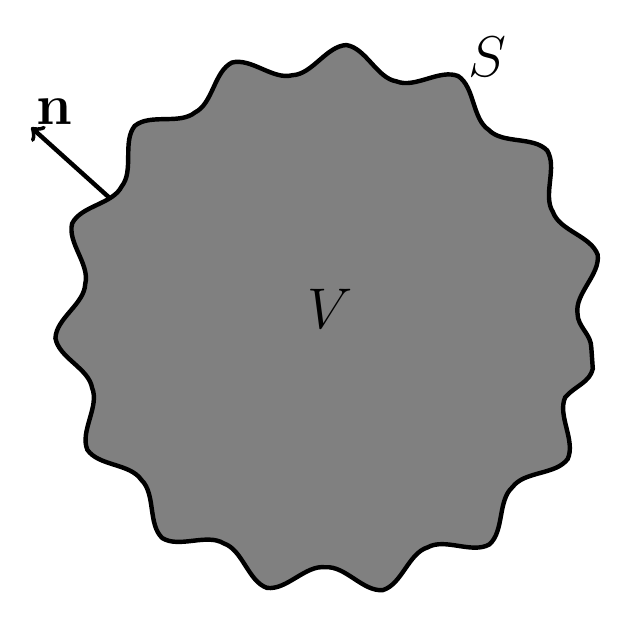
\begin{tikzpicture}[ultra thick]
		\draw(0,0) node[circle,decorate, decoration={snake,amplitude=5pt,segment length=40pt},draw,scale=20,fill=gray]{};
		%\draw(0,0) node[star,star points=7,decorate, decoration=random steps,star point ratio=0.8,draw,scale=20,fill=gray]{};
	          \draw(2,3.7)node{\huge$S$};
	           \draw(0,0.5)node{\huge$V$};
	            \draw[->](-2.8,1.9)--(-3.8,2.8);
	           \draw(-3.5,3)node{\huge$\mathbf{n}$};
\end{tikzpicture}
\end{document}
